Las once parejas de distancias están en la tabla \ref{tab:distancias}. Además de los valores medidos se incluye la diferencia $\Delta = s_o - s_i$ y el error relativo de cada medición, calculado como
\begin{equation}
E = \frac{\left| s_o - s_i \right|}{s_o} \times 100 ,
\label{eq:error}
\end{equation}
tomando $s_o$ como referencia, porque según la ecuación \eqref{eq:distancias} es el valor que debería tener $s_i$.

\begin{center}
\begin{tabular}{ccccc}
\hline
Posición & $s_o$ (cm) & $s_i$ (cm) & $\Delta$ (cm) & $E$ \\
\hline
1  & 21.0 & 20.5 & 0.5 & 2.38 \\
2  & 12.8 & 12.5 & 0.3 & 2.34 \\
3  & 8.0  & 7.6  & 0.4 & 5.00 \\
4  & 18.2 & 18.0 & 0.2 & 1.10 \\
5  & 24.8 & 24.7 & 0.1 & 0.40 \\
6  & 12.5 & 12.2 & 0.3 & 2.40 \\
7  & 24.7 & 24.5 & 0.2 & 0.81 \\
8  & 18.0 & 17.8 & 0.2 & 1.11 \\
9  & 7.9  & 7.7  & 0.2 & 2.53 \\
10 & 12.2 & 12.1 & 0.1 & 0.82 \\
11 & 20.8 & 20.7 & 0.1 & 0.48 \\
\hline
\end{tabular}
\captionof{table}{Distancia objeto, distancia imagen, su diferencia y el error relativo en por ciento para cada posición.}
\label{tab:distancias}
\end{center}

A primera vista los números de las dos columnas son casi iguales. La diferencia nunca pasó de medio centímetro, y en promedio fue de
\begin{equation}
\bar{\Delta} = 0.24 \pm 0.13 \text{ cm},
\label{eq:promedio}
\end{equation}
mientras que el error relativo promedio fue de 1.8 por ciento, con un máximo de 5 por ciento en la posición 3.

Para verlo de forma gráfica se colocó $s_i$ contra $s_o$ en la figura \ref{fig:grafica} y se ajustó una recta por mínimos cuadrados:
\begin{equation}
s_i = 1.005 \, s_o - 0.32 ,
\label{eq:ajuste}
\end{equation}
con un coeficiente de determinación $R^2 = 0.9996$.

\begin{center}
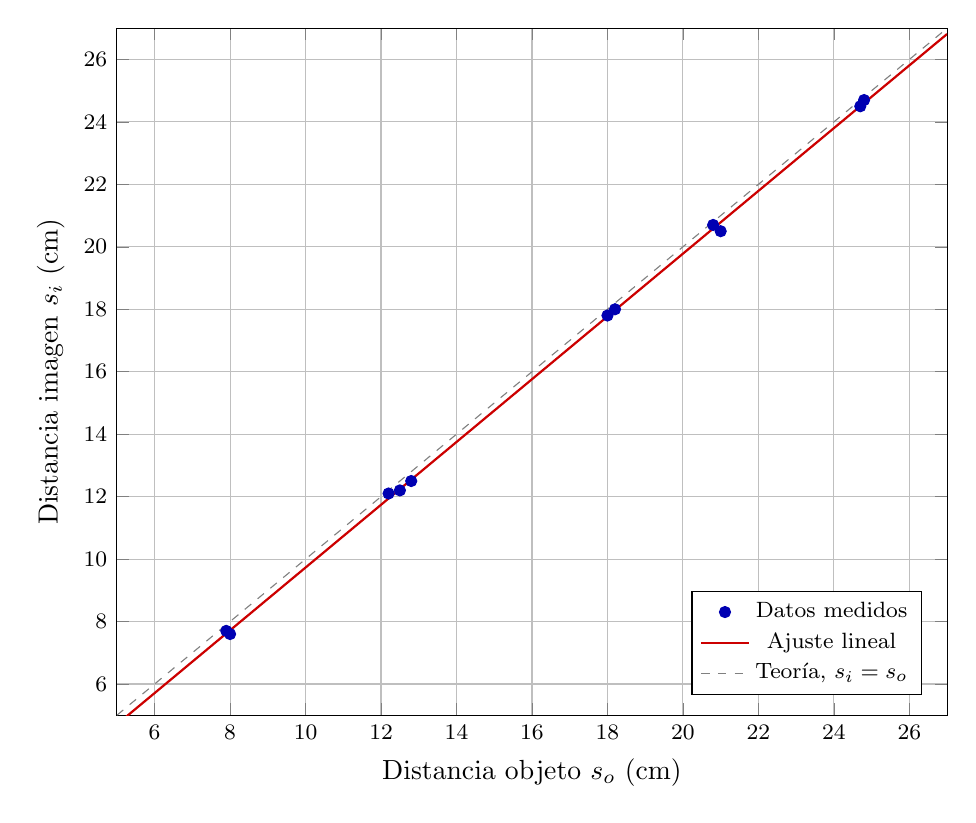
\begin{tikzpicture}
\begin{axis}[
    width=\columnwidth,
    height=0.85\columnwidth,
    xlabel={Distancia objeto $s_o$ (cm)},
    ylabel={Distancia imagen $s_i$ (cm)},
    xmin=5, xmax=27,
    ymin=5, ymax=27,
    grid=major,
    legend pos=south east,
    legend style={font=\footnotesize},
    tick label style={font=\footnotesize},
]
\addplot[only marks, mark=*, color=blue!70!black] coordinates {
    (21.0,20.5) (12.8,12.5) (8.0,7.6) (18.2,18.0) (24.8,24.7) (12.5,12.2)
    (24.7,24.5) (18.0,17.8) (7.9,7.7) (12.2,12.1) (20.8,20.7)
};
\addlegendentry{Datos medidos}
\addplot[domain=5:27, samples=2, thick, color=red!80!black] {1.005*x - 0.32};
\addlegendentry{Ajuste lineal}
\addplot[domain=5:27, samples=2, dashed, color=gray] {x};
\addlegendentry{Teoría, $s_i = s_o$}
\end{axis}
\end{tikzpicture}
\captionof{figure}{Distancia imagen contra distancia objeto. La recta roja es el ajuste de la ecuación \eqref{eq:ajuste} y la línea punteada es la predicción teórica.}
\label{fig:grafica}
\end{center}

Las dos rectas casi se enciman. Además, en el pliego de la figura \ref{fig:trazo} se nota que cada imagen quedó a la misma altura que su objeto, sobre la misma perpendicular al espejo.
